\documentclass[a4paper]{ctexart}
\usepackage{ctex}
\usepackage{xcolor}
\pagestyle{plain}
\usepackage{geometry}
\geometry{left=3.0cm, right=3.0cm, top=2.0cm, bottom=2.0cm}
\usepackage{graphics}
\usepackage{hyperref}
\usepackage{amsmath}
\title{编译实习课程改革\ 实习报告}
\date{}
\author{李汪洋\ 李佳蔚\ 梁家硕}
\ctexset{section/format = {\Large\bfseries}}
\hypersetup{
colorlinks=true,
linkcolor=black
}

\begin{document}

\maketitle
\tableofcontents
\newpage

\section{编译实习课程}

\subsection{编译课程概览}

目前北京大学的编译原理(编译技术)课程与编译实习课程,是形式上独立而实际上紧密结合的两门课程。编译原理主要讲授理论,编译实习主要动手实践。

编译原理课程前半学期主要讲:正则表达式与自动机、词法分析、上下文无关的语法分析、语法制导翻译。后半学期主要讲:中间代码生成、运行时环境、寄存器分配、代码优化。

编译实习课程的任务是实现一个MiniJava的编译器,以巩固编译原理课程上学到的知识。总体流程是:MiniJava $\rightarrow$ Piglet $\rightarrow$ Spiglet $\rightarrow$ Kanga $\rightarrow$ MIPS。

\subsection{MiniJava任务的一些缺陷}

由于课程内容设计和选课系统的一些原因,还无法将这两门课合并成一门课,而且两门课程在进度上有些不协调。由于编译原理与编译实习两课程联系紧密,同学们通常在同一学期同时选修这两门课程。根据之前同学们的反映,两门课经常出现进度差异问题,比如实习课要用到的技术在原理课上还没有讲,实习课前半学期基本只做前端工作导致后半学期工作量过大等等。

MiniJava任务是同学单人完成,同学们可能头一次面对这样的大项目,做起来可能有些吃力。但对于一些能力较强的同学,也可能觉得任务有些简单。

在MiniJava编译器整体任务由词法分析、语法分析、寄存器分配等多个小任务组成,小任务间环环相扣,同学们如果在之前的某一环没有完成好,可能影响之后代码编写和完成进度。

另外,编译课程不要求先修Java程序设计,而MiniJava虽然语法不复杂,但其编译器要求用Java实现,对于没有接触过Java的同学有些不友好。

\subsection{课程改革}

我们设计出一套全新的MiniC编译器框架,以替代当前编译实习课程使用的MiniJava,来解决编译课程目前面临的一系列问题。并希望能与信息科学技术学院的体系结构实习、操作系统实习等课程的改革结合,帮助学生更好地理解计算机科学与技术。

编译实习课程改革的目标主要有三点。

一,在一定程度上降低门槛,让能力不太强的同学也能顺利完成任务,体验编译器的编写流程,对于能力较强的同学,提供一些可选的扩展内容。

二,尽可能配合编译原理课程进度,更合理地进行任务分配。

三,使任务模块化,单独对某一阶段知识点进行实践测试,对于先前已经做完的任务,提供标准模块,避免项目前面遗留问题对后期进度的影响。

\newpage
\section{MiniC编译器}

\subsection{概述}

MiniC编译器的目标是把MiniC语言一步一步转化成合法的32位RISC-V汇编。

MiniC编译器,除了MiniC语言外,还涉及Eeyore和Tigger两种中间语言,和最终要输出的RISC-V汇编。

MiniC编译器总共有3个必要大步骤,总体流程是:MiniC $\rightarrow$ Eeyore $\rightarrow$ Tigger $\rightarrow$ RISC-V。

MiniC, Eeyore, Tigger的设计都遵循简洁易读的原则,方便同学处理。同学们没必要使用Eeyore或Tigger的全部语法,如果觉得使用它们的某个子集就能完成任务也是可以的。%(其实我们认为Eeyore和Tigger已经高度精简,没必要再取子集了)

Eeyore和Tigger这两个名称,继承了MiniJava编译器中使用到的Piglet和Kanga的命名传统。都取自同一动画``Winnie Pooh"。

\begin{center}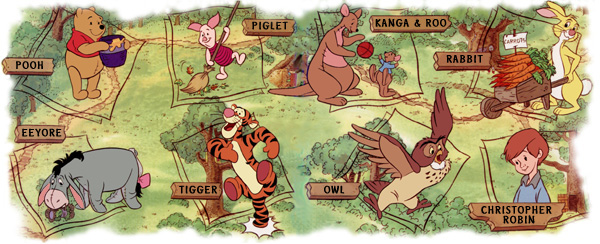
\includegraphics[width=15cm]{name} \end{center}

据了解,以往同学们MiniJava编译器编写时遇到的困难主要有三点:课程进度问题、类型检查复杂琐碎、寄存器分配算法有难度。我们的解决方案分别是,重新安排课程进度使之与原理课程匹配,减少数据类型的数量,推荐一些更好写的寄存器分配算法(相比原理课上讲的图染色法)。

\subsection{MiniC}

MiniC是C语言的一个子集,我们对C语言进行了大量的删减,力图产生一种高度精简的、易于实现的语言。对于MiniC的语言定义与描述,参考《MiniC文档说明》。

MiniC编译器的第一步,是实现MiniC语言的词法分析和语法分析(可以利用lex和yacc等工具),并分析语义,将MiniC转换成Eeyore中间语言。

MiniC的类型只有int和一维int数组,极大地减小了类型检查的工作量。

\subsection{Eeyore}

Eeyore是一中三地址码,为了让同学们易于接受,Eeyore的语法是编译原理课程教学用书(龙书)中使用的三地址码格式的扩展。具体描述参考《Eeyore文档说明》。

Eeyore可以看作是MiniC编译器中的Piglet和Spiglet。

在这一步,要做的是优化(可选)和寄存器分配工作。输入Eeyore代码,输出Tigger格式的中间代码。

\subsection{* 优化}

优化阶段不是必须的,有能力的同学可以选做。在考核方面,可单独对产出的Eeyore的运行速度进行测试。

编译优化阶段的输入和输出格式都是Eeyore。

\subsection{Tigger}

Tigger可以被认为是Eeyore进行了寄存器分配后的版本,与Eeyore语法很像。具体描述参考《Tigger文档说明》。

Tigger可以看作是MiniC编译器中的Kanga。

在这一步,要做的是把Tigger代码转换为RISC-V汇编。这几乎是一句对应一句的简单文本处理了。

\subsection{RISC-V}

生成合法的RISC-V汇编之后,同学们要做的所有工作就完成了。

我们会调用riscv-gcc把生成的RISC-V汇编转成机器码。

最终使用RISC-V的模拟器运行机器码,并进行最终的整体测试。(中间步骤的完成情况使用我们编写的Eeyore和Tigger模拟器进行阶段性测试)

\subsection{进度安排}

根据我们小组完成各阶段所用的时间,我们对同学们的MiniC编译器任务做了如下初步进度安排。(我们小组的完成进度在下一节)

第1--2周:努力学习编译原理,并预习语法制导翻译部分,并尝试学习安装riscv-gcc。

第3--7周:完成MiniC$\rightarrow$Eeyore。具体地说,第3周实现符号表与类型检查,第4周完成词法分析,第5周完成文法书写,第6周处理表达式翻译,第7周处理控制流翻译。

第8--11周:完成Eeyore$\rightarrow$Tigger。具体地说,第8周完成Eeyore的语法树构建,第9周实现活性分析,第10周实现寄存器分配,第11周输出Tigger代码。

第12--13周:完成Tigger$\rightarrow$RISC-V。包括熟悉RISC-V汇编和输入输出格式处理。

第14周:编写实验报告。

可以看出,以上时间安排没有占满整个学期的时间,这是考虑到同学们有期中期末考试以及假期,预留出了2周左右的时间。根据我们自己的经验,主要的难度在于Eeyore和Tigger的产生,而最后一步相对比较容易,所以还可以有一周时间用于活动安排或者用于扩展内容或程序优化。

\newpage
\section{工作完成情况}

\subsection{MiniC方面}
\begin{itemize}
	\item 完成MiniC语法制定
	\item 完成MiniC的parser
\end{itemize}

前半学期花了很多时间实现了复杂MiniC语法的parser,几乎是把所有扩展内容都实现了。

parser使用on-the-f\/ly翻译模式,维护了一个极复杂但表达能力很强的符号表,如果只是翻译base语法集可以删去很多没必要的类型与检查。

parser编写过程中遇到了C语言中不区分布尔表达式与其他表达式的问题,这会使原理课上学的回填技术无法使用。为了解决这个问题parser放弃了回填技术,但仍用on-the-f\/ly翻译模式,只是先计算表达式的值,然后再进行逻辑判断。这样做使得遇到逻辑表达式时产出的代码略冗长,但确实解决了问题,也能正确处理\texttt{||}与\texttt{\&\&}短路跳转。为了让同学们方便处理,base语法集限定布尔表达式不可以是算术表达式。

另外,C语言的文法(用lex和yacc表示的)可以直接从网上找到,我们希望同学们能自己完成MiniC文法的编写,不要直接抄网上现成的lex和yacc代码。

\subsection{Eeyore方面}

\begin{itemize}
	\item 完成Eeyore语法制定
	\item 完成Eeyore模拟器
	\item 完成Eeyore上的寄存器分配算法,把Eeyore转化成Tigger
\end{itemize}

即使是在已经简化过的 Eeyore 文法上,也是较为复杂一步。预处理使用了 lex + yacc,建出符号表。寄存器分配使用了 Linear Scan 算法,相较于之前的 web + 图染色算法,大大简化。

这步比较麻烦的是在最后生成 Tigger 代码的时候,会有许多特殊情况。寄存器与变量之间的关系较为混乱,稍有不慎就会写错。另一个难点是处理数组,这里需要对数组,地址等概念非常清晰。

处理种种特殊情况时,为了代码实现的更简明一些,在某些细节上会产生一些浪费现象。处理这些细节也是一个有技术难度的工作,可以考虑作为扩展内容。

关于 Linear Scan 算法的详细说明,详见 Linear Scan 的说明文档。

\subsection{Tigger方面}

\begin{itemize}
	\item  完成Tigger语法制定
	\item  完成Tigger模拟器
	\item  完成Tigger转为RICS-V汇编
\end{itemize}

Tigger模拟器的实现,先利用lex和yacc构建语法树(其实基本是一条链),在运行之前给全局变量赋值,然后从\texttt{f\_main}开始执行,执行过程中维护栈和寄存器的值。

由于Tigger语法很简单,模拟器实现起来没什么困难。

Tigger模拟器同Eeyore模拟器一样,也实现了调试功能,帮助同学们调试寄存器分配算法。
\\

\subsection{评测方面}
\begin{itemize}
	\item 完成测试平台搭建
	\item 完成测试程序以及测试数据构造
\end{itemize}

测试程序都是些MiniC程序,这些程序有大有小,可以比较全面地对编译器的正确性和产出代码的质量进行测试。但是因为我们对编译测试的原理不太熟悉,所以测试程序可能设计的有一些缺陷,这一点我们可以之后进一步修正。

对于每个MiniC测试程序,我们都构造了一些测试数据,每个测试数据包括一个输入文件和一个答案文件。

我们没有专门构造Eeyore和Tigger的测试集,因为同学们有可能不会用到Eeyore和Tigger的全部语法。因此,Eeyore和Tigger的测试程序应由MiniC的测试程序经过转化而来,测试数据与之前的相同。

评测平台我们使用的是CMU开源的Autolab测试平台,也就是我们学校著名的ICS课程使用的测试平台,实现在线测评和统计成绩。

\subsection{计划与现实}

说实话,没想到选编译实习课程改革这个题目会有这么大的任务量,时间很紧张。虽然每个小任务的不太难,但任务数量很多。

按照开题时的计划,期中前基本要把完整的编译器做出来,期中后实现一些工具和测试脚本,设置扩展内容。

事实上,在期中前,我们用了大量时间设计了一套比现在看到的复杂得多的MiniC和三地址码,并完成实现了它们的parser和模拟器。

中期报告后紧接着的一两周,小组三人都忙于各种考试与其他任务,没时间写代码。在老师与助教的指点下,意识到同学们不太可能实现这么复杂的语法,就在这段时间制定了一套从头到尾全新的MiniC,Eeyore,Tigger语法,明确了之后要做的工作。

现在看来,在期中前我们相当于实现了大部分扩展内容,体验了一把复杂的扩展内容是多么难写。

最后的几周,完成的工作比较多。为提供运行效率重写了Eeyore模拟器。为了减轻同学们的负担,也为了小组能尽快完成任务,学习并实现了Linear Scan寄存器分配算法。编写了Tigger模拟器。测试程序和测试数据集,搭建了测试平台。

\newpage
\section{写给后来人}

在实践过程中,我们深切体会到课程改革之不易。我们的工作也许只是改革的一个开端,想真正投入教学,还需实践检验。我们在这里记录下编译实习课程改革的一些经验,希望能对之后投身这项课程改革的人们有些许启发。
\\

Eeyore模拟器和Tigger模拟器可作为测试工具提供给同学,完成的MiniC编译器的三大步骤的代码,可以用作标准模块。

如果不使用标准模块,同学们可以只使用Eeyore和Tigger语言的一个子集,把自己产出的那个子集翻译好就可以正确地产生RISC-V代码了。如果同学在前面的某个步骤没能顺利完成,那么把标准模块提供给他时,他可能会面临标准模块产出的代码超出了他原本使用的那个子集这样的问题。

我们小组只保证标准模块之间能正确拼接成一个正确的编译器,同学们写的模块与标准模块拼接时可能会出现不兼容的问题,因为我们目前手上只有自己写的标准模块,还无法做这方面的测试工作。
\\

MiniC语法扩展内容,也许无法被翻译成Eeyore或Tigger代码,这是因为Eeyore和Tigger是专门为MiniC的base语法集制定的,无法表达一些base以外的语法。所以对于想做MiniC语法扩展内容的同学,只能对扩展内容单独测试,同学们要想办法把扩展的部分最终转成RISC-V,比如可以自行扩展Eeyore和Tigger的语法使它们支持扩展内容。
\\

同学们若想本地测试自己生成的RISC-V汇编是否正确,需要先下载并编译riscv-tools,再利用riscv-gcc生成机器码,最后用RISC-V的模拟器来运行。在我们小组编译riscv-tools的过程中,遇到了大量奇怪的编译错误,RISC-V官方并没有给出多少对于这些编译错误的说明,致使我们花费了不少时间来解决这些错误。我想同学们在尝试编译riscv-tools的时候,也许会觉得很头大。

\end{document}
